\documentclass[
10pt, % Main document font size
a4paper, % Paper type, use 'letterpaper' for US Letter paper
oneside, % One page layout (no page indentation)
%twoside, % Two page layout (page indentation for binding and different headers)
headinclude,footinclude, % Extra spacing for the header and footer
BCOR5mm, % Binding correction
]{scrartcl}

\usepackage{listings}
\usepackage{color}
%\usepackage{biblatex}

\definecolor{dkgreen}{rgb}{0,0.6,0}
\definecolor{gray}{rgb}{0.5,0.5,0.5}
\definecolor{mauve}{rgb}{0.58,0,0.82}

\lstset{frame=tb,
	language={},
	aboveskip=3mm,
	belowskip=3mm,
	showstringspaces=false,
	columns=flexible,
	basicstyle={\small\ttfamily},
	numbers=none,
	numberstyle=\tiny\color{gray},
	keywordstyle=\color{blue},
	commentstyle=\color{dkgreen},
	stringstyle=\color{mauve},
	breaklines=true,
	breakatwhitespace=true,
	tabsize=3
}

\usepackage{german}


%usepackage[utf8]{inputenc}
%\usepackage{geometry}
\usepackage[german,onelanguage,linesnumbered, ruled]{algorithm2e}
\SetAlFnt{\small}
\SetAlCapFnt{\large}
\SetAlCapNameFnt{\large}
%\usepackage{algpseudocode}


%%%%%%%%%%%%%%%%%%%%%%%%%%%%%%%%%%%%%%%%%
% Arsclassica Article
% Structure Specification File
%
% This file has been downloaded from:
% http://www.LaTeXTemplates.com
%
% Original author:
% Lorenzo Pantieri (http://www.lorenzopantieri.net) with extensive modifications by:
% Vel (vel@latextemplates.com)
%
% License:
% CC BY-NC-SA 3.0 (http://creativecommons.org/licenses/by-nc-sa/3.0/)
%
%%%%%%%%%%%%%%%%%%%%%%%%%%%%%%%%%%%%%%%%%

%----------------------------------------------------------------------------------------
%	REQUIRED PACKAGES
%----------------------------------------------------------------------------------------

\usepackage[
nochapters, % Turn off chapters since this is an article        
beramono, % Use the Bera Mono font for monospaced text (\texttt)
eulermath,% Use the Euler font for mathematics
pdfspacing, % Makes use of pdftex’ letter spacing capabilities via the microtype package
dottedtoc % Dotted lines leading to the page numbers in the table of contents
]{classicthesis} % The layout is based on the Classic Thesis style

\usepackage{arsclassica} % Modifies the Classic Thesis package

\usepackage[T1]{fontenc} % Use 8-bit encoding that has 256 glyphs

\usepackage[utf8]{inputenc} % Required for including letters with accents

\usepackage{graphicx} % Required for including images
\graphicspath{{Figures/}} % Set the default folder for images

\usepackage{enumitem} % Required for manipulating the whitespace between and within lists

\usepackage{lipsum} % Used for inserting dummy 'Lorem ipsum' text into the template

\usepackage{subfig} % Required for creating figures with multiple parts (subfigures)

\usepackage{amsmath,amssymb,amsthm} % For including math equations, theorems, symbols, etc

\usepackage{varioref} % More descriptive referencing

%----------------------------------------------------------------------------------------
%	THEOREM STYLES
%---------------------------------------------------------------------------------------

\theoremstyle{definition} % Define theorem styles here based on the definition style (used for definitions and examples)
\newtheorem{definition}{Definition}

\theoremstyle{plain} % Define theorem styles here based on the plain style (used for theorems, lemmas, propositions)
\newtheorem{theorem}{Theorem}

\theoremstyle{remark} % Define theorem styles here based on the remark style (used for remarks and notes)

%----------------------------------------------------------------------------------------
%	HYPERLINKS
%---------------------------------------------------------------------------------------

\hypersetup{
%draft, % Uncomment to remove all links (useful for printing in black and white)
colorlinks=true, breaklinks=true, bookmarks=true,bookmarksnumbered,
urlcolor=webbrown, linkcolor=RoyalBlue, citecolor=webgreen, % Link colors
pdftitle={}, % PDF title
pdfauthor={\textcopyright}, % PDF Author
pdfsubject={}, % PDF Subject
pdfkeywords={}, % PDF Keywords
pdfcreator={pdfLaTeX}, % PDF Creator
pdfproducer={LaTeX with hyperref and ClassicThesis} % PDF producer
} % Include the structure.tex file which specified the document structure and layout

\hyphenation{Fortran hy-phen-ation} % Specify custom hyphenation points in words with dashes where you would like hyphenation to occur, or alternatively, don't put any dashes in a word to stop hyphenation altogether

%----------------------------------------------------------------------------------------
%	TITLE AND AUTHOR(S)
%----------------------------------------------------------------------------------------

\title{\normalfont\spacedallcaps{Projektaufgabe AE}} % The article title

\subtitle{Remove Duplicates - Spotify playlist cleaner} % Uncomment to display a subtitle

\author{\spacedlowsmallcaps{Raphael Drechsler}} % The article author(s) - author affiliations need to be specified in the AUTHOR AFFILIATIONS block

\date{} % An optional date to appear under the author(s)

%----------------------------------------------------------------------------------------

\begin{document}

%----------------------------------------------------------------------------------------
%	HEADERS
%----------------------------------------------------------------------------------------

\renewcommand{\sectionmark}[1]{\markright{\spacedlowsmallcaps{#1}}} % The header for all pages (oneside) or for even pages (twoside)
%\renewcommand{\subsectionmark}[1]{\markright{\thesubsection~#1}} % Uncomment when using the twoside option - this modifies the header on odd pages
\lehead{\mbox{\llap{\small\thepage\kern1em\color{halfgray} \vline}\color{halfgray}\hspace{0.5em}\rightmark\hfil}} % The header style

\pagestyle{scrheadings} % Enable the headers specified in this block

%----------------------------------------------------------------------------------------
%	TABLE OF CONTENTS & LISTS OF FIGURES AND TABLES
%----------------------------------------------------------------------------------------

%\maketitle % Print the title/author/date block
{ \centering
{ \par}\
 \linebreak
\linebreak 
\linebreak
\linebreak
\linebreak
%\centering

\includegraphics[width=0.55\columnwidth]{htwLogo} 
\linebreak
\linebreak
\linebreak
\linebreak 
 % inline
{\fontsize{14}{16}\selectfont \center Fakultät Informatik, Mathematik und\\Naturwissenschaften\\Studiengang Informatik Master\par}\
 \linebreak
{\fontsize{18}{20}\selectfont \center \textbf{Projektarbeit zur Vorlesung Computermusik}\par}\
{\fontsize{20}{22}\selectfont \center \textbf{BrandtBrauerFrick.hs} \par}\
\linebreak
\linebreak
\linebreak
\linebreak 
\linebreak
\linebreak 
\linebreak 
{\fontsize{14}{16}\selectfont  \begin{tabular}{rl}
 	\textbf{Autoren:} & Nico Mehlhose, Raphael Drechsler\\ 
 	\textbf{Abgabedatum:} & 01.02.2019 \\ 
 \end{tabular}
\par}
\par}
\pagebreak
\setcounter{tocdepth}{2} % Set the depth of the table of contents to show sections and subsections only

%\tableofcontents % Print the table of contents
%\listoffigures % Print the list of figures
%\listoftables % Print the list of tables




%----------------------------------------------------------------------------------------

\newpage % Start the article content on the second page, remove this if you have a longer abstract that goes onto the second page

%----------------------------------------------------------------------------------------
%	INTRODUCTION
%----------------------------------------------------------------------------------------
\section{Abstract}\
\textit{Abschnitt bearbeitet von: Raphael Drechsler}\\

\noindent \textbf{BrandtBrauerFrick.hs}

\noindent Brandt Brauer Frick ist ein Techno-Projekt aus Berlin.
Die Basis des Projekts bilden Klänge aus dem Instrumentarium der
klassischen Musik, welche anfangs gesampelt, später in einem zehnköpfigen
Ensemble auch live vorgeführt wurden.\cite{Wiki}\\ 

\noindent Ziel des Projektes:\\
Die Umsetzung des Songs ''Pretend'' von Brandt Brauer Frick entweder in
Tidal oder Euterpea. Eine online verfügbare Live-Aufführung \cite{YT1} soll dabei als Refernz dienen. Bei der Umsetzung soll auch Wert auf die Nachbildung der echten Instrumente und deren teilweise Zweckentfremdung gelegt werden.\\

\noindent Herausforderungen:
\begin{itemize}
	\itemsep0em
	\item Evaluation ob Tidal oder Euterpea genutzt werden soll:
	\item Untersuchung der Frage ob klassische Klänge am ehesten in Euterpea oder
	Tidal nutzbar sind. (Durch repetitiven Charakter des Liedes würde sich Tidal zur
	Live-Vorführung eignen)
	\item Analyse der einzelnen musikalischen Bausteine und deren Implementierung.
	\item Zusammenfügen der erarbeiteten Bausteine zu einer Performance.
\end{itemize}

\section{Tidal oder Euterpea}\
\textit{Abschnitt bearbeitet von: Nico Mehlhose}\\

\noindent Dieses Thema soll sich um die Evaluation zwischen Tidal und Eutherpea handeln.\\
Unsere Entscheidung Tidal zu nehmen beruht gewiss nicht auf einer zufälligen Entscheidung. In diese Entscheidung ist der Programmieraufwand, vorhandenen Informationen
und die Möglichkeit den Synthesizer zu erweitern.\\
Bei dem Programmieraufwand wird sehr schnell klar, dass durch das Lied \textit{Pretent} von BrandBrauerFrick Tidal besser geeignet ist als Euterpea. Der erste Gesichtspunkt
der betrachtet wurde ist die Repetetivität des Songs, welcher in Euterpea zwar auch umsetzbar ist aber in Tidal von Anfang an gegeben ist, da Tidal die Sounds immer in einem
Loop abspielt. Bei den vorhandenen Informationen stellt sich heraus, dass es keine Offiziellen Notenblätter für das Lied Onlinegibt, wodurch Euterpea etwas an Bedeutung verliert, da Euterpea für genaue Notenbestimmungen perfekt geeignet wäre. Da dieser Fakt aber nicht vorliegt, kann das selbe Maß an Genauigkeit auch mit Tidal erreicht werden.\\
Der letzte und für uns wichtigste Punkt war die Erweiterbarkeit der Sounds. Die Wichtigkeit darin besteht in der entfremdeten Benutzung der Musikinstrumente in dem Lied.
In Eutherpea haben wir nach einiger Recherche keinen weg gefunden Sounds hinzuzufügen um diese später zu verwenden. In Tidal allerdings existiert diese Möglichkeit mittels
des Befehl \textit{}. Mit diesem Befehl lässt sich ein Verzeichnis in Tidal integrieren.
%~dirt.loadSoundFiles("full/path/to/directory/*") noch in textit einfügen
\section{Analyse des Stücks Pretend - Allgemein}\
\textit{Abschnitt bearbeitet von: Raphael Drechsler}\\

\noindent Die in der Live vorgeführte Version \cite{YT1} hat eine ungefähre Dauer von 7 Minuten, 15 Sekunden. Die Angabe erfolgt ungefähr, da die Aufnahme nicht mit dem ersten Takt beginnt\\
Das Stück steht in der Tonart Gm.\\
Über ein BPM-Measuring-Tool \cite{tempo} wurde ein Tempo von 130bpm ermittelt. In Tidal wird somit der folgende Code zur Tempo-Einstellung benötigt. 
\begin{lstlisting}
setcps (130/60/4)
\end{lstlisting}

\noindent Um die Globale Struktur des Liedes, also die Zeitliche Abfolge der Figuren der einzelnen Instrumente zu visualisieren, wurden in einer DAW leere MIDI-Blöcke innerhalb der 237 Takte erzeugt und dann F1,F2,... für die jeweilige Figur beschriftet.\\
Dabei wurden für die ersten vier Takte eine Annahme getroffen.

\begin{figure}[h]
	\centering 
	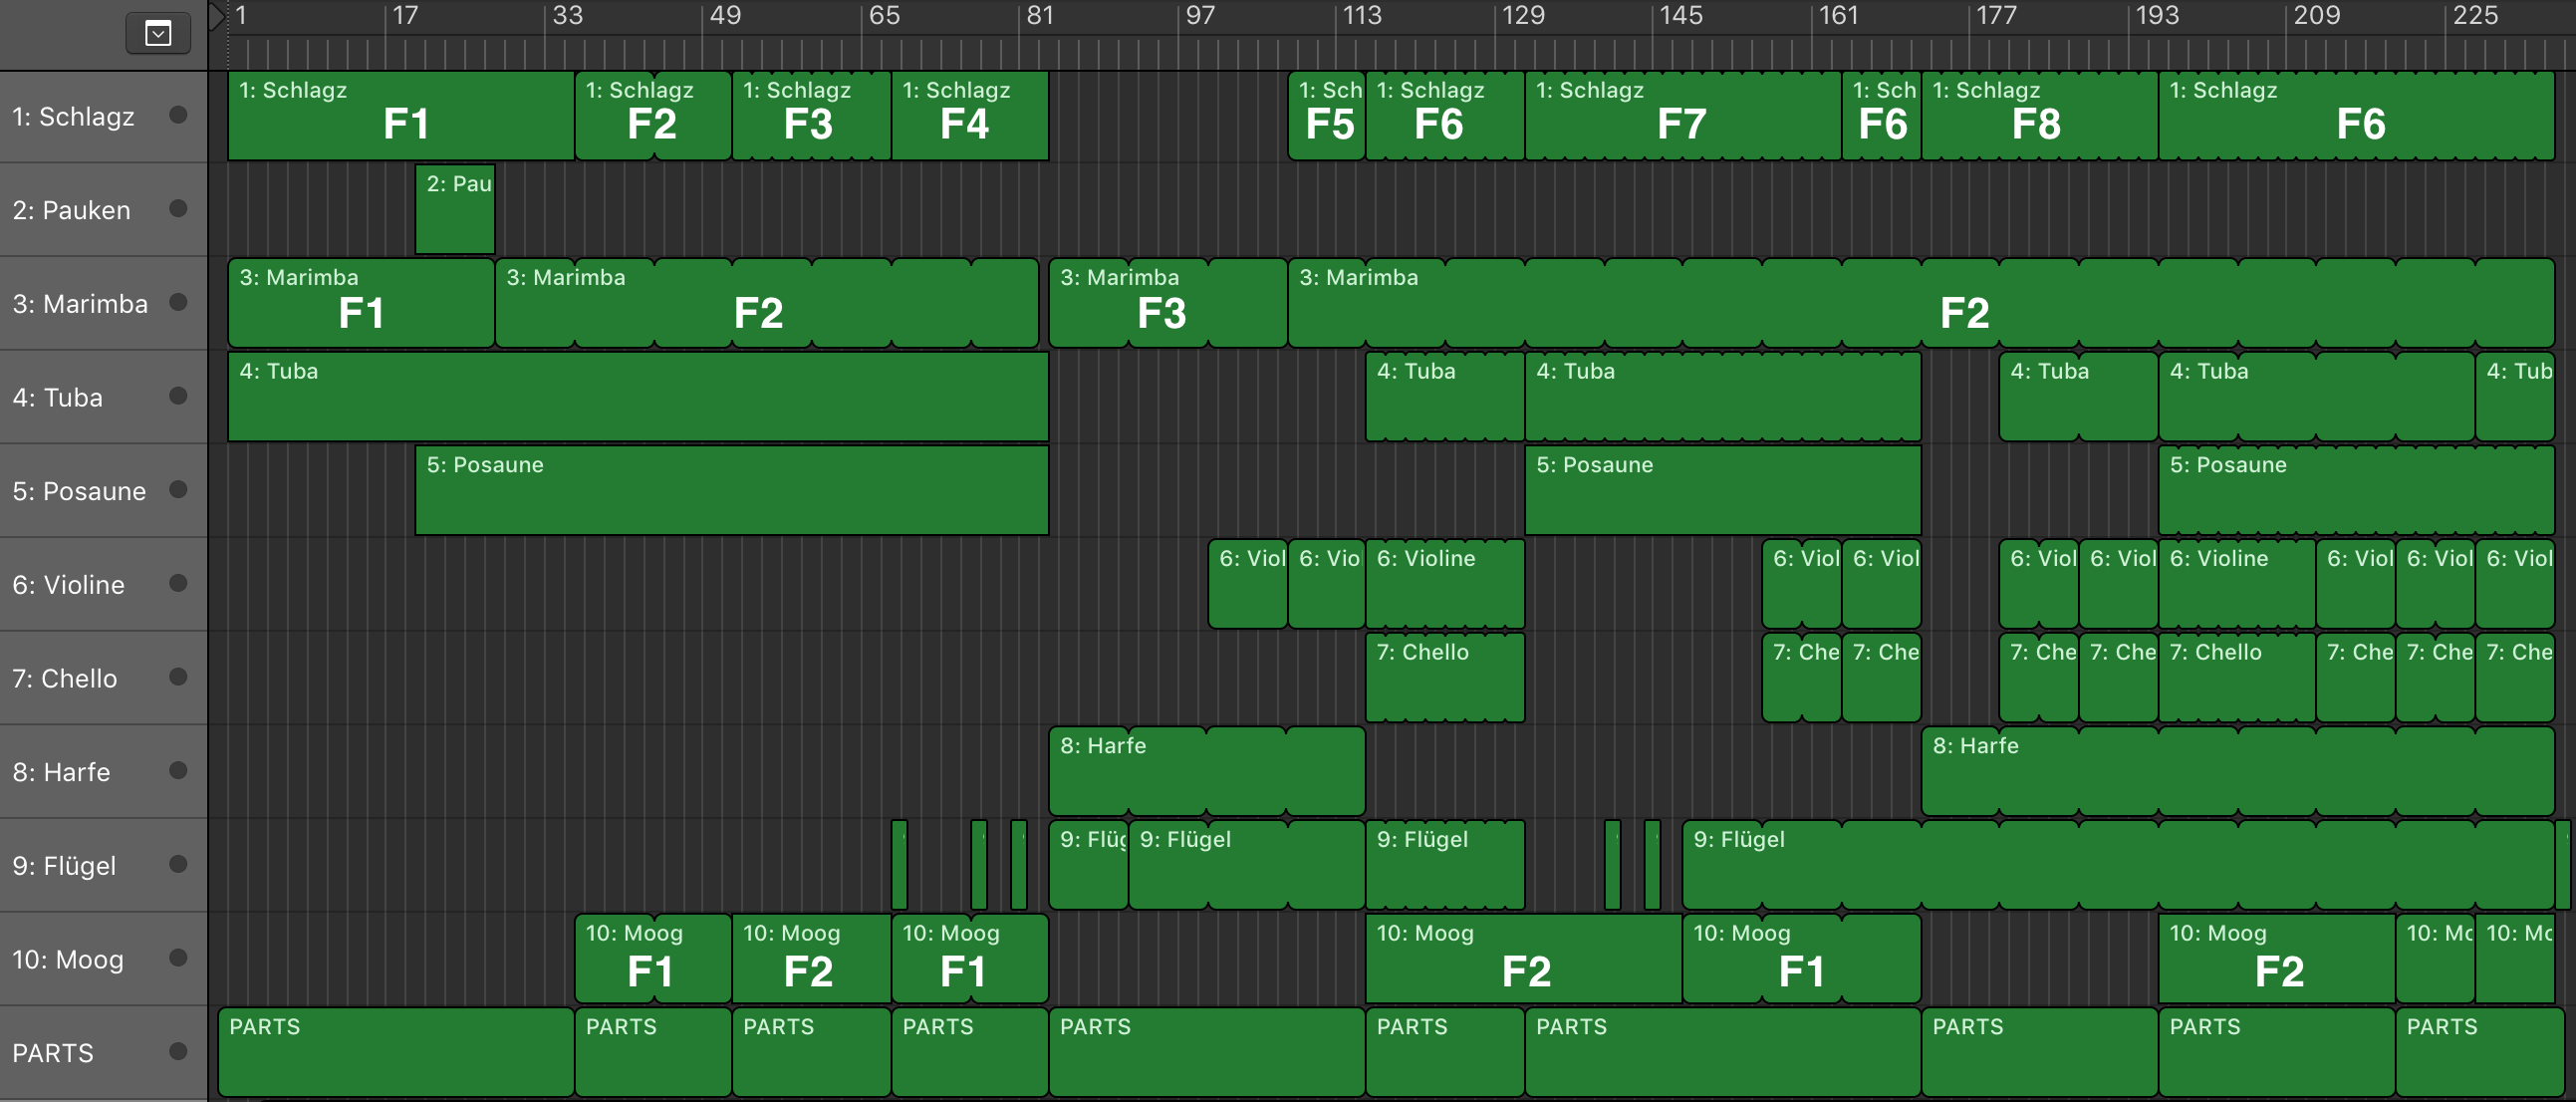
\includegraphics[width=0.99\columnwidth]{GlobaleStrukturMarkiert} 
	\caption{Globale Struktur dargestellt als leere MIDI-Regionen in DAW mit Beschriftung der Figuren}
\end{figure}

\noindent Es wurde ebenfalls versucht die Abfolge mithilfe eines freien Notations-Programmes in einer Partitur darzustellen. Jedoch erwies sich die obige Darstellung als kompakter und ausreichend.

\section{Analyse des Stücks Pretend}\
Im folgenden Abschnitt sollen die zehn Instrumente untersucht werden. Dabei sind pro Instrument die folgenden Fragen zu klären:

\begin{itemize}
	\itemsep0em
	\item Welche Figuren werden gespielt?
	\item Wie sind die einzelnen Figuren zu spielen?
	\item Welcher Klänge werden pro Figur vom Instrument gespielt?
	\item Wie lassen sich diese Klänge in den jeweiligen Figuren nachbilden?
\end{itemize}

%
%\subsection{Instrument 0: Was ist pro Instrument TODO?}
%{\color{red}\textbf{TODO}}: Nach Bearbeitung Hilfskapitel entfernen.\\
%
%Raph.\\
%Welche Figuren?
%- Welche Wirkung?
%- Welche Noten?\\
%
%Nico\\
%Wie klingt das Instrument?\\
%- Wie klingt das live? Einzelne Bestandteile? (Marimba gespielt mit Holzsticks und verschiedene Kuhglocken)
%- Wie klingt das in welcher Figur? (zB. BD laut, leise)
%- Welchen Klang wählen (evaluation - SD-Instrument nutzbar?, WAV suchen/selber aufnehmen, Instrument coden)\\

\subsection{Instrument 1: Schlagzeug}
\subsubsection{Figuren}
\textit{Abschnitt bearbeitet von: Raphael Drechsler}\\

\noindent \textbf{Figur 1}\\
Treibender Grundrhythmus, Base-Drum und High-Hat im Wechsel. Dabei über mehrere Takte ansteigende Lautstärke der Base-Drum.
\begin{figure}[h]
	\centering 
	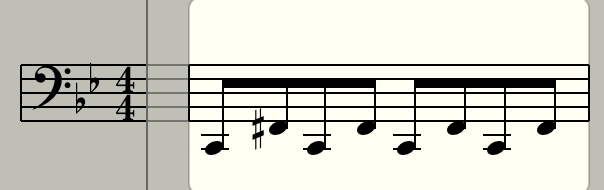
\includegraphics[width=0.35\columnwidth]{Drum_Fig1} 
	\caption{Schlagzeug Figur 1}
\end{figure}

\begin{lstlisting}
d1 $ sound "[bd hh]*4"
\end{lstlisting}

\noindent \textbf{Figur 2}\\
Analog zu Figur 1. Dabei mehr Fills auf die High-Hat\\
{\color{red}\textbf{TODO}} Noten, Code oder Absicht und Programmlogik\\

\noindent \textbf{Figur 3}\\
Analog zu Figur 1 und 2. Dabei noch mehr Fills auf die High-Hat\\
{\color{red}\textbf{TODO}} Noten, Code oder Absicht und Programmlogik\\

\noindent \textbf{Figur 4}\\
Analog zu Figur 1. Dazu kommen zyklische Bewegung auf der Rim (Rand der Snare-Drum).
Die Figur ließ sich nur schwer durch Raushören bestimmen. Es wurden daher 5 Schläge auf die Rim pro Takt als Annahme getroffen, wobei aller 2 Takte der letzte Schlag ausgelassen wird.

\begin{lstlisting}
d1 $ slow 2 $ stack [
sound "[bd hh]*8",
fastcat[sound "[rm rm rm rm rm]", sound "[rm rm rm rm ~]"]
]
\end{lstlisting}

\noindent \textbf{Figur 5}\\
Nur die zyklische Rimclick-Bewegung aus Figur 4.
\begin{lstlisting}
d1 $ slow 2 $ fastcat[sound "[rm rm rm rm rm]", sound "[rm rm rm rm ~]"]
\end{lstlisting}

\noindent \textbf{Figur 6}\\
Wie Figur 4, aber kräftig gespielt.\\

\noindent \textbf{Figur 7}\\
Ähnlich zu Figur 3. Treibender Rhythmus, viele Fills.\\
{\color{red}\textbf{TODO}} Noten, Code oder Absicht und Programmlogik\\

\noindent \textbf{Figur 8}\\
Wie Figur 4 aber ohne Base-Drum.
\begin{lstlisting}
d1 $ slow 2 $ stack [
sound "[~ hh]*8",
fastcat[sound "[rm rm rm rm rm]", sound "[rm rm rm rm ~]"]
]
\end{lstlisting}

\subsubsection{Klangbild}
\textit{Abschnitt bearbeitet von: Nico Mehlhose}\\

\noindent Bestandteile des Schlagzeuges: herkömmliches Schlagzeug\\
Art der Synthetisierung: Da Bass Drum und High Head normal gespielt werden können die Sounds aus dem Supercollider 
mit minimaler Anpassung benutzt werden. Lediglich die Rim aus Figur 4 muss, wegen ihres hölzernen Sounds, selbst 
aufgenommen werden.
\noindent \textbf{Figur 1}\\
Sound BD: Base Drum wird mit zunehmender dauer lauter gespielt\\
Sound HH: wird Anfangs nur sanft angespielt aber mit zunehmender Zeit etwas lauter\\
Problem: Base Drum und High Heads müssen mit zunehmender Vorführungszeit lauter werden\\ 
Lösung:\\
\begin{lstlisting}
Code: d1 $ slow 2 $ sound "[bd hh]*8" #gain "<0.7 0.9 1.1 1.3>"
\end{lstlisting}

Fig4:\\
Sound Rim:\\
Nico: selber bauen da keine hölzernen klänge vorhanden sind

Fig6:\\
irgendwas mit gain?\\



Töne: hh, bd (dumpf, wenig knackig)\\
rim

\subsection{Instrument 2: Pauken}
\subsubsection{Figuren}
{\color{red}\textbf{OFFEN}} \\
{\color{red}\textbf{TODO}}
(Hierzu Studio-Version hören)\\

\subsubsection{Klangbild}
3 Kesselpauken

\subsection{Instrument 3: Marimba}
\subsubsection{Figuren}
{\color{red}\textbf{OFFEN}} \\
{\color{red}\textbf{TODO}}\\
Aufbau beschreiben mit Glocken.\\
Random-Funktion benötigt

\subsubsection{Klangbild}
Holzsticks auf Marimba in verschiednenen Tonhöhen wobei eher rhythmisch als melodisch eingesetzt, dazu Kuh-Glocken bereitstellen für Random-Funktion

\subsection{Instrument 4: Tuba}
\subsubsection{Figuren}
\textit{Abschnitt bearbeitet von: Raphael Drechsler}\\

\noindent\textbf{Figur 1}\\
Figur über einen Takt. Schlag auf Tuba-Mundstück als rhythmisches Element auf zweite Zählzeit im Takt.\\
\begin{figure}[h]
	\centering 
	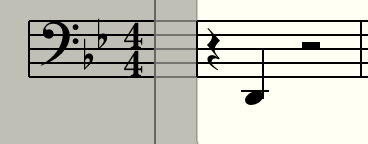
\includegraphics[width=0.25\columnwidth]{Tuba_Fig1} 
	\caption{Tuba Figur 1}
\end{figure}

\begin{lstlisting}
d1 $ sound "[~ sn ~ ~]"
\end{lstlisting}

\subsubsection{Figuren}
\textbf{Figur 2}\\
Figur über 2 Takte. Instrumentalist bläst in die Tuba ohne dass die Lippen vibrieren, um ein Rauschen zu erzeugen. Pause am Ende der Figur als Atempause angenommen. 

\begin{figure}[h]
	\centering 
	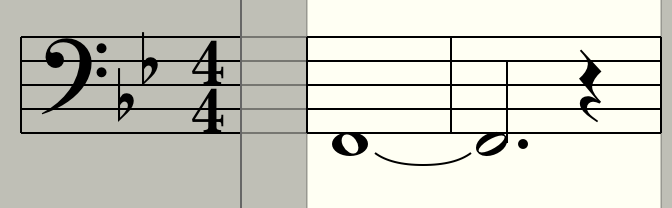
\includegraphics[width=0.25\columnwidth]{Tuba_Fig2} 
	\caption{Tuba Figur 2}
\end{figure}

\begin{lstlisting}
--Idee: sound, der 2 Takte dauert alle 2 Takte 1x anpsielen
d1 $ sound "blasesoundTuba"
\end{lstlisting}

\noindent\textbf{Figur 3}\\
Wie Figur 1, hier allerdings kurzes tonloses Pusten stoßweise gespielt anstelle von Schlag auf Mundstück.\\

\noindent\textbf{Figur 4}\\
Tiefe Töne durch Tuba, Tonhöhe nicht entscheidend und fast nicht mehr wahrnehmbar. Ein Gefühl von Bedrohung wird beim Hörer erzeugt. Der Ton ''rollt'' langsam an\\
{\color{red}\textbf{TODO}} Noten, Code\\

\noindent\textbf{Figur 5}\\
Wie Figur 4, kräftig ausgespielt.\\

\noindent\textbf{Figur 6}\\
Wie Figur 5, maximal kraftvoll ausgespielt. Eine Oktave höher gespielt daher Tonhöhe der einzelnen Töne gut erkennbar.\\
{\color{red}\textbf{TODO}} Code

\subsubsection{Klangbild}
\textit{Abschnitt bearbeitet von: Nico Mehlhose}\\

\noindent Bestandteile der Tuba: normale Tuba, welche aber entartet benutzt wird\\
Art der Synthetisierung: Da die Tuba ein reales Musikinstrument ist, welches in dieser Form nicht im Supercollider enthalten ist,
werden hierfür Samples benutzt. Die Samples werden für die entartete Benutzung in Tidal so manipuliert, dass sie die Sounds
nachempfinden.\\
Für Figur 2 werden eigene Samples aufgenommen. Den Sound soll ein Handscheibenwischer mit einem hohlen Griff erzeugen.

\noindent\textbf{Figur 1}\\
 Sound: In dieser Figur wird auf das Mundstück der Tuba geschlagen. Der erzeugte Ton hört sich in etwa an wie eine Base Drum ohne Bass.\\
Lösung:\\
\begin{lstlisting}
d1 $ sound "~ bd ~ ~" # midinote 15
\end{lstlisting}

\noindent\textbf{Figur 2}\\
Sound: ähnlich eines Reifens der Luft verliert\\
Lösung:\\
\begin{lstlisting}
Nico: d1 $ sound "[sax ~ ~ hh]" # speed 0.35 # midinote 55 # gain "[1 0]" # cut 1 \\
d1 $ sound "[trump ~ ~ hh]" # speed 0.05 # midinote 55 # gain "[0.7 0]" # cut 1\\
\end{lstlisting}

\noindent\textbf{Figur 3}\\
Sound: Wie Sound aus Figur 2 aber mit mehr Druck und nicht durchgehend.\\
Lösung:\\


\subsection{Instrument 5: Posaune}
\subsubsection{Figuren}
\textit{Abschnitt bearbeitet von: Raphael Drechsler}\\

\noindent\textbf{Figur 1}\\
Figur über einen Takt. Kurzes, tonloses Pusten in die Posaune. Stoßweise gespielt als rhythmisches Element auf letzte Achtelnote im Takt.\\
\begin{figure}[h]
	\centering 
	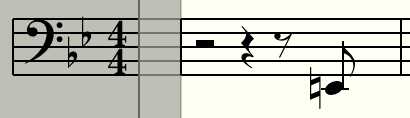
\includegraphics[width=0.25\columnwidth]{Posaune_Fig1} 
	\caption{Posaune Figur 1}
\end{figure}

\begin{lstlisting}
d1 $ sound "[][[][~ sn]]"
\end{lstlisting}


\noindent\textbf{Figur 2}\\
Erzeugen von Rauschen analog zu Figur 2 - Tuba. Dabei Lautstärke zum Ende des Stückes hin zunehmend.
\begin{lstlisting}
--Idee: sound, der 2 Takte dauert alle 2 Takte 1x anpsielen
--Frage: Lautstaerke?
d1 $ sound "blasesoundPosaune"
\end{lstlisting}

\subsubsection{Klangbild}
Bestandteile derPosaune: normale Posaune, welche aber entartet benutzt wird\\
Art der Synthetisierung: Da die Posaune ein reales Musikinstrument ist, welches in dieser Form nicht im Supercollider enthalten ist,
werden hierfür Samples benutzt. Die Samples werden für die entartete Benutzung in Tidal so manipuliert, dass sie die Sounds
nachempfinden.\\
Für Figur 2 werden eigene Samples aufgenommen. Den Sound soll ein Handscheibenwischer mit einem hohlen Griff erzeugen.

\noindent\textbf{Figur 1}\\
 Sound: In dieser Figur wird auf das Mundstück der Posaune stoßartig angespielt.\\
Lösung:\\
\begin{lstlisting}
\\
\end{lstlisting}

\noindent\textbf{Figur 2}\\
Sound: ähnlich zu Figur 3 der Tuba allerdings mit weniger tief.\\
Lösung:\\
\begin{lstlisting}
\\
\end{lstlisting}

\subsection{Instrument 6: Violine}
\subsubsection{Figuren}
\textit{Abschnitt bearbeitet von: Raphael Drechsler}\\

\noindent\textbf{Figur 1}\\
Leicht schrill gespielte Figur mit gebrechlicher, wimmernder Wirkung. Die Figur wird gegen Ende Lauter und steigt in der Tonhöhe und erzeugt somit einen anwachsenden Spannungsbogen im Hörgefühl.
\begin{figure}[h]
	\centering 
	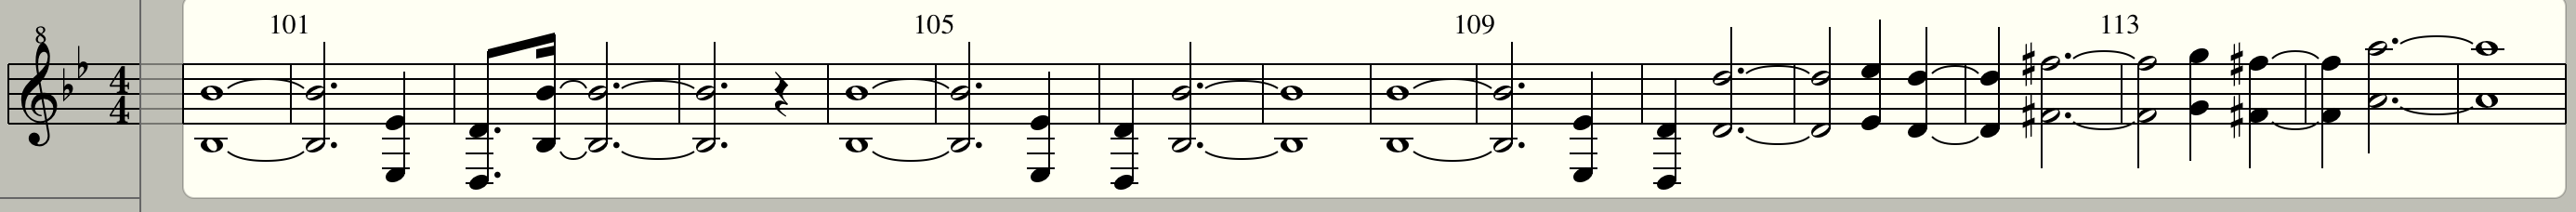
\includegraphics[width=0.99\columnwidth]{Violin_Fig1} 
	\caption{Violine Figur 1}
\end{figure}

\noindent Die Noten der Figur werden oktaviert gespielt. Der Einfachheit halber wurden nur dir gut hörbaren hohen töne umgesetzt.

\begin{lstlisting}
p "i6" $ slow 16 $ fastcat [
midinote "[82][][][][][][][75][74][82][][][][][][]" # s "gtr",
midinote "[82][][][][][][][75][74][82][][][][][][]" # s "gtr",
midinote "[82][][][][][][][75][74][86][][][][][87][86]" # s "gtr",
midinote "[][90][][][][][91][90][][93][][][][][][]" # s "gtr"
] # room 0.85 # sz 0.8 # orbit 1 #gain 0.9
\end{lstlisting}\

\noindent\textbf{Figur 2}\\
In Tonhöhe abfallende, schnelle Figur, die Bewegung erzeugt. Diese wird im Vibrato gespielt, was die Bewegung intensiviert.
\begin{figure}[h]
	\centering 
	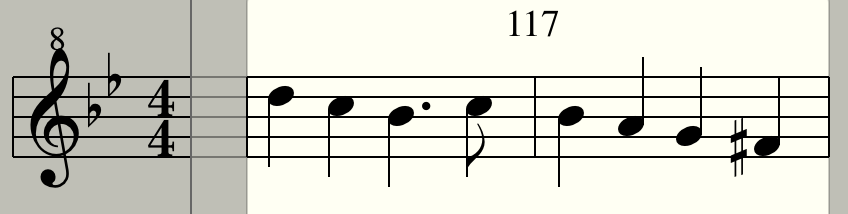
\includegraphics[width=0.3\columnwidth]{Violin_Fig2} 
	\caption{Violine Figur 2}
\end{figure}

\begin{lstlisting}
p "i6" $ slow 2 $ midinote "[[86][84][82][[][84]]][82 81 79 78]" # s "gtr"
\end{lstlisting}

\noindent\textbf{Figur ?}\\
{\color{red}\textbf{TODO}} weitere Figuren im hinteren Teil des Stückes

\subsubsection{Klangbild}
Ruhige Parts, Hektik (schnell gespielte Töne)\\
gegebenenfalls aus Toenen aus Samples zusammensetzen und nicht durch midinotes


\subsection{Instrument 7: Chello}
\subsubsection{Figuren}
\textit{Abschnitt bearbeitet von: Raphael Drechsler}\\

\noindent\textbf{Figur 1}\\
Untermalt die bewegungsvolle Figur 2 der Violine. Ist dabei ebenso bewegungsvoll und ebenfalls mit Vibrato gespielt um den Effekt zu intensivieren.
\begin{figure}[h]
	\centering 
	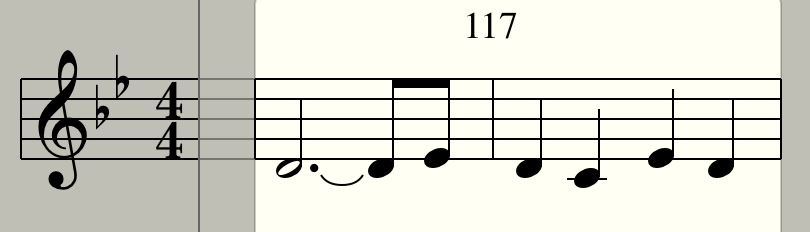
\includegraphics[width=0.3\columnwidth]{Chello_Fig1} 
	\caption{Chello Figur 1}
\end{figure}

\begin{lstlisting}
p "i7" $ slow 2 $ midinote "[[74][][][[][75]]][74 72 75 74]" # s "gtr"
\end{lstlisting}

\noindent\textbf{Figur 2}\\
{\color{red}\textbf{TODO}} \\

\noindent\textbf{Figur ?}\\
{\color{red}\textbf{TODO}} weitere Figuren im hinteren Teil des Stückes

\subsubsection{Klangbild}
Ruhige Parts, Hektik (schnell gespielte Töne)


\subsection{Instrument 8: Harfe}
\subsubsection{Figuren}
\textit{Abschnitt bearbeitet von: Raphael Drechsler}\\

\noindent\textbf{Figur 1}\\
{\color{red}\textbf{TODO}} Starke Annahme - hier vllt was mit Random aus Skala nehmen machen.
\begin{figure}[h]
	\centering 
	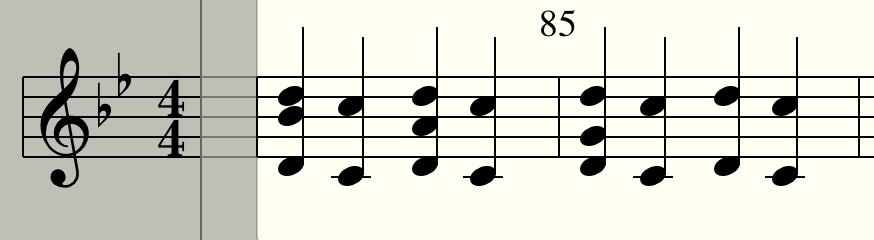
\includegraphics[width=0.3\columnwidth]{Harp_Fig1} 
	\caption{Harfe Figur 1}
\end{figure}

\begin{lstlisting}
d1 $ slow 2 $ stack [
	midinote "[74 72]*4" # s "gtr", 
	midinote "[62 60]*4" # s "gtr", 
	slow 2 $ fastcat [
		midinote "70 69" # s "gtr", 
		midinote "67" # s "gtr",
		midinote "70 69" # s "gtr", 
		midinote "66" # s "gtr"    
	]
]
\end{lstlisting}



\subsubsection{Klangbild}
...

\subsection{Instrument 9: Flügel}
\subsubsection{Figuren}
\textit{Abschnitt bearbeitet von: Raphael Drechsler}\\

\noindent\textbf{Figur 1}\\
Nur ein Tiefer Ton.
\begin{figure}[h]
	\centering 
	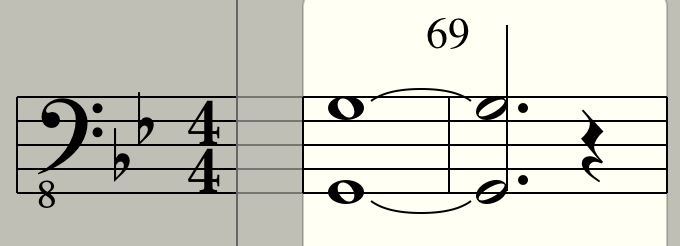
\includegraphics[width=0.3\columnwidth]{Flug_Fig1} 
	\caption{Flügel Figur 1}
\end{figure}

\begin{lstlisting}
p "i9" $ slow 2 $ stack[midinote "43 " #s "superpiano", midinote "55 " #s "superpiano"]
\end{lstlisting}

\noindent \textbf{Figur 2}\\
Zwei gleichzeitig, kurz angespielte Töne.
\begin{figure}[h]
	\centering 
	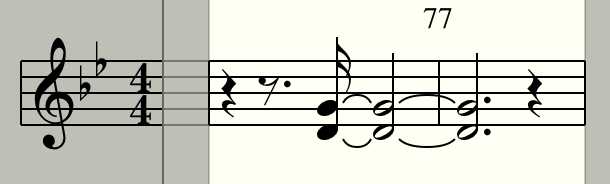
\includegraphics[width=0.3\columnwidth]{Flug_Fig2} 
	\caption{Flügel Figur 2}
\end{figure}\\
{\color{red}\textbf{TODO}} Code\\


\noindent \textbf{Figur 3}\\
{\color{red}\textbf{TODO}}Beschreibung\\
\begin{figure}[h]
	\centering 
	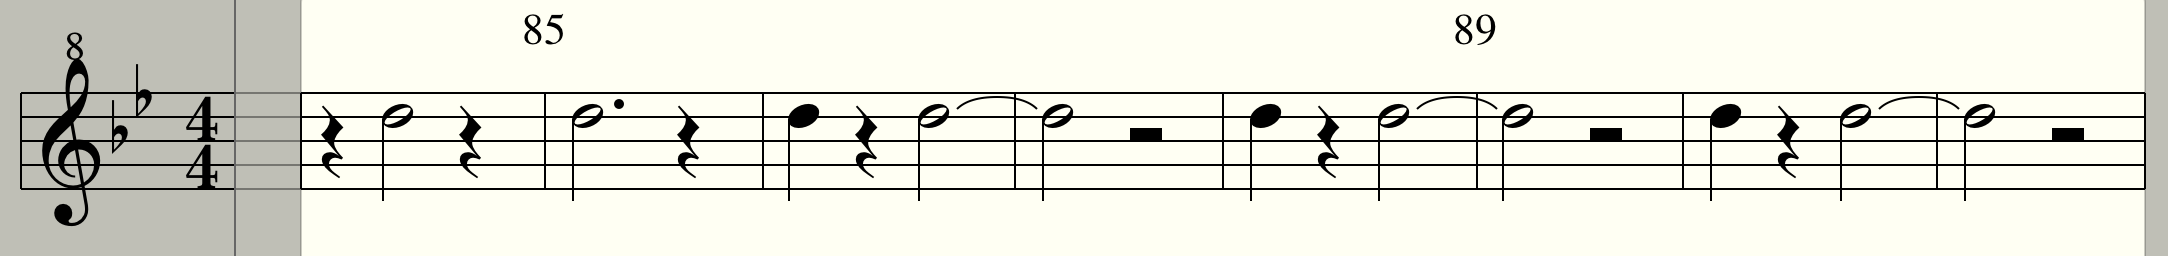
\includegraphics[width=0.8\columnwidth]{Flug_Fig3} 
	\caption{Flügel Figur 3}
\end{figure}
\begin{lstlisting}
p "i9" $ slow 2 $ midinote "[86 ~][86][~] [~] " # s "superpiano"  # room 0.5 # sz 0.83 # orbit 1 #gain "<0.65 0.7 0.75 0.8>"
\end{lstlisting}


\noindent \textbf{Figur 4}\\
{\color{red}\textbf{TODO}}Beschreibung\\
\begin{figure}[h]
	\centering 
	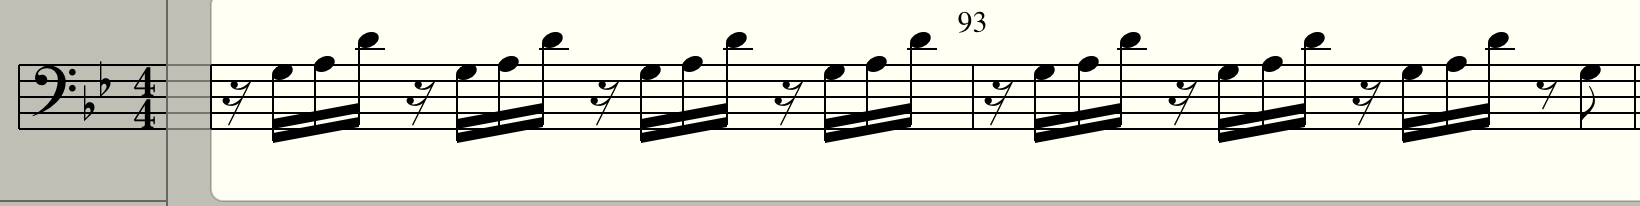
\includegraphics[width=0.9\columnwidth]{Flug_Fig4a} 
	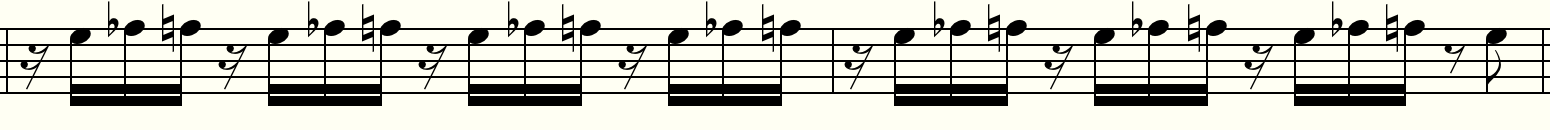
\includegraphics[width=0.9\columnwidth]{Flug_Fig4b} 
	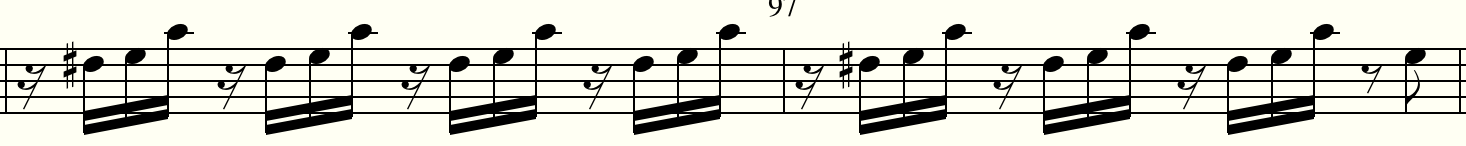
\includegraphics[width=0.9\columnwidth]{Flug_Fig4c} 
	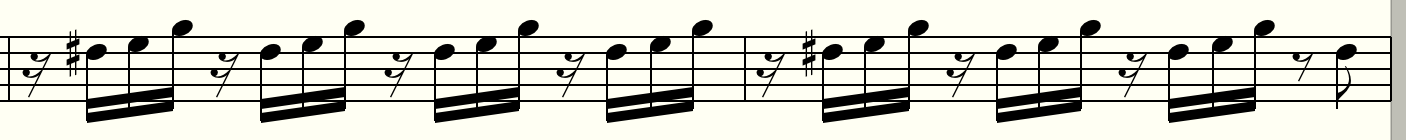
\includegraphics[width=0.9\columnwidth]{Flug_Fig4d} 
	\caption{Flügel Figur 4}
\end{figure}
\begin{lstlisting}
d1 $ slow 8 $ fastcat [
midinote "~ 67 69 74 ~ 67 69 74 ~ 67 69 74 ~ 67 69 74 ~ 67 69 74 ~ 67 69 74 ~ 67 69 74  ~ ~ 67 ~ " # s "superpiano",
midinote "~ 67 68 69 ~ 67 68 69 ~ 67 68 69 ~ 67 68 69 ~ 67 68 69 ~ 67 68 69 ~ 67 68 69  ~ ~ 67 ~ " # s "superpiano",
midinote "~ 66 67 72 ~ 66 67 72 ~ 66 67 72 ~ 66 67 72 ~ 66 67 72 ~ 66 67 72 ~ 66 67 72  ~ ~ 67 ~ " # s "superpiano",
midinote "~ 66 67 70 ~ 66 67 70 ~ 66 67 70 ~ 66 67 70 ~ 66 67 70 ~ 66 67 70 ~ 66 67 70  ~ ~ 66 ~ " # s "superpiano"
]
\end{lstlisting}

\noindent \textbf{Figur 5}\\
{\color{red}\textbf{TODO}}Beschreibung\\
\begin{figure}[h]
	\centering 
	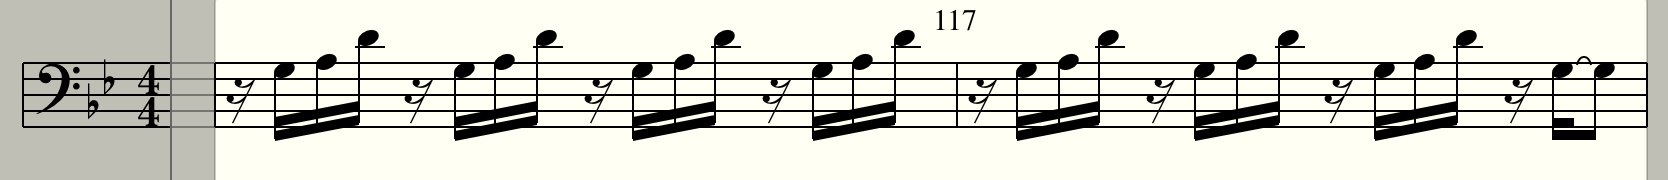
\includegraphics[width=0.9\columnwidth]{Flug_Fig5} 
	\caption{Flügel Figur 5}
\end{figure}
\begin{lstlisting}
d1 $ slow 2 $ midinote "~ 67 69 74 ~ 67 69 74 ~ 67 69 74 ~ 67 69 74 ~ 67 69 74 ~ 67 69 74 ~ 67 69 74  ~ ~ 67 ~ " # s "superpiano"
\end{lstlisting}


\subsubsection{Klangbild}
...


\subsection{Instrument 10: Moog Syntheziser}
\subsubsection{Figuren}
\textit{Abschnitt bearbeitet von: Raphael Drechsler}\\

\noindent\textbf{Figur 1}\\
Basslauf über 8 Takte.\\
{\color{red}\textbf{TODO}}Bessere Beschreibung\\
\begin{figure}[h]
	\centering 
	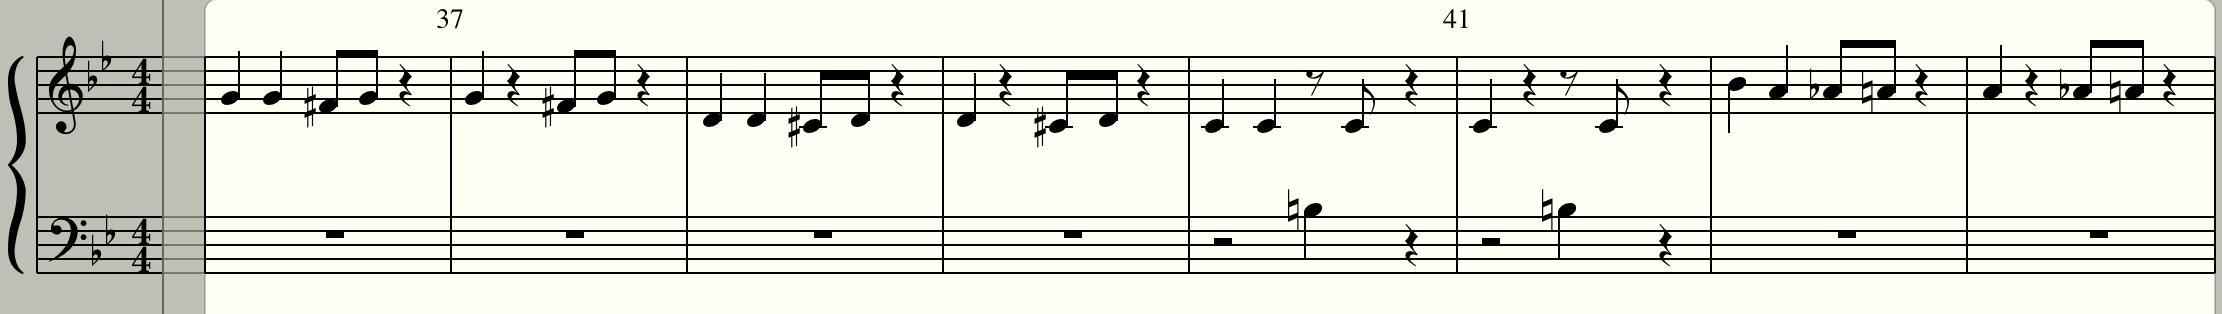
\includegraphics[width=1\columnwidth]{Bass_Fig1} 
	\caption{Moog Figur 1}
\end{figure}

\begin{lstlisting}
---Arbeitsstand
--2Takte
d1 $ midinote "[[55 55][54 55 ~ ~]]" # s "moog" # cut 1
--2Takte
d1 $ midinote "[[50 50][49 50 ~ ~]]" # s "moog" # cut 1
--2Takte
d1 $ midinote "[[48 48][47 48 ~ ~]]" # s "moog" # cut 1
--1 Takte
d1 $ midinote "[[58 57][56 57 ~ ~]]" # s "moog" # cut 1
--1 Takte
d1 $ midinote "[[57 ~][56 57 ~ ~]]" # s "moog" # cut 1

---Verbunden:
d1 $ slow 8 $ fastcat [midinote "[[55 55][54 55 ~ ~]]*2" # s "moog" # cut 1,
midinote "[[50 50][49 50 ~ ~]]*2" # s "moog" # cut 1,
midinote "[[48 48][47 48 ~ ~]]*2" # s "moog" # cut 1,
midinote "[[58 57][56 57 ~ ~]]  [[57 ~][56 57 ~ ~]]" # s "moog" # cut 1
]
\end{lstlisting}

\noindent\textbf{Figur 2}\\
Basslauf über einen Takt.\\
{\color{red}\textbf{TODO}}Beschreibung\\
\begin{figure}[h]
	\centering 
	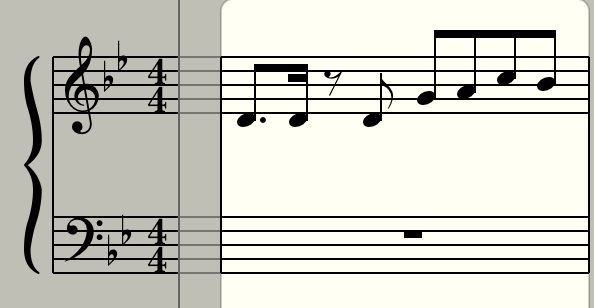
\includegraphics[width=0.3\columnwidth]{Bass_Fig2} 
	\caption{Moog Figur 2}
\end{figure}

\begin{lstlisting}
---Arbeitsstand
d1 $ midinote "[[[[50 ~ ~ 50]][~ 50]][55 57 60 58]]" # s "moog" # cut 1
\end{lstlisting}



\subsubsection{Klangbild}
...

\section{Performance}
TODO:\\
Spuren per Stack verbinden?\\
Konzept für Ablauf Performance?\\
Wie mehrtaktige Figuren mit every zusammenfassen?
Link zu den Soundfiles: http://virtualplaying.com/virtual-playing-orchestra/ \\
https://rhythm-lab.com/moog-rogue-bass/

\pagebreak

%----------------------------------------------------------------------------------------
%	BIBLIOGRAPHY
%----------------------------------------------------------------------------------------

\renewcommand{\refname}{\spacedlowsmallcaps{Literatur/Quellen}} % For modifying the bibliography heading

\bibliographystyle{unsrt}

\bibliography{biblo.bib} % The file containing the bibliography

%----------------------------------------------------------------------------------------

\end{document}